\documentclass[12pt,a4paper,oneside, titlepage]{report}

\usepackage{times}
\usepackage[french,frenchb]{babel}
%\usepackage{hyperref}
\usepackage[utf8]{inputenc}
\usepackage[T1]{fontenc}
%\usepackage{amsmath}
%\usepackage{amsfonts}
%\usepackage{amscd}
%\usepackage{amstext}
%\usepackage{amssymb}
%\usepackage{bar}
\usepackage{color}
%\usepackage{mathrsfs}
\usepackage{graphicx}
%\usepackage{calligra}
\usepackage{amsthm}
%\usepackage{multirow}
%\usepackage{tabularx}
%\usepackage{layout}
%\pagestyle{headings}
\usepackage{fancyhdr}
\usepackage{array}
\usepackage{lscape}
\usepackage{rotating}
\usepackage[style=alphabetic,sortcites=true,block=space]{biblatex}
% \usepackage{pstricks}
\usepackage{pstricks}
\usepackage{csquotes}
\pagestyle{fancy}

\bibliography{biblio}

\setlength{\textheight}{630pt}
\setlength{\footskip}{30pt}
\newtheorem{defi}{D\'efinition}[section]
\newtheorem{note}{Note}[section]
\newtheorem{propriete}{Propri\'et\'e}[section]
\newtheorem{exemple}{Exemple}[section]
\newtheorem{exemple_util}{Exemple d'utilisation}
\newtheorem{corollaire}{Corollaire}[section]
\newtheorem{rem}{Remarque}[section]
\newtheorem{thm}{Th\'eor\`eme}[section]
\newtheorem{illustration}{Illustration}[section]
\newenvironment{demonstration}{\begin{proof}[\textnormal{\textbf{Preuve.}}]}{\end{proof}}
\definecolor{gris}{gray}{0.45}
\setlength{\parindent}{1cm}
\newcommand{\textcalli}[1]{{\small{\textbf{$\negmedspace$\calligra #1}}}}
\interfootnotelinepenalty=10000

% \renewcommand{\chaptermark}[1]{\markright{\thechapter\ #1}}
\renewcommand{\sectionmark}[1]{\markright{\thesection\ #1}}
\fancyhf{} % supprime les en-têtes et pieds prédéfinis
\fancyhead[R]{\thepage}% Left Even, Right Odd
\fancyhead[L]{\textsl{\leftmark}} % Left Odd
%\fancyhead[RE]{\textsl{\leftmark}} % Right Even
\renewcommand{\headrulewidth}{0pt}% filet en haut de page
\renewcommand{\footrulewidth}{0pt} % pas de filet en bas
\fancypagestyle{plain}{ % pages de tetes de chapitre
\fancyhead{} % supprime l'entete
\fancyhead[R]{\thepage}
\renewcommand{\headrulewidth}{0pt} % et le filet
}

\begin{document}
%newpage
\thispagestyle{empty}
%\null
%\newpage
\begin{titlepage}
% \vspace*{0.95cm}
\begin{center}
\textnormal{\Large{Universit\'e de Mons}}\\[0.3em]
\textnormal{\Large{Facult\'e des Sciences}}\\[0.3em]
\textnormal{\Large{Institut d'Informatique}}\\[0.3em]
\end{center}
\vspace*{4cm}
\begin{center}
\fbox{
\begin{minipage}{14cm}
\center
\vspace*{0.5cm}\textbf{\LARGE{Copier/coller multi-plateformes}}
\vspace*{0.4cm}
\end{minipage}
}
\end{center}
\vspace*{3cm}

\large{
\begin{center}
\begin{tabular*}{14.5cm}{@{\extracolsep{\fill}}lr}
Directeur : M\textsuperscript{r} Olivier \textsc{Delgrange} &
Projet r\'ealis\'e par\\
& Maëlick \textsc{Claes}\\[1em]
Rapporteurs : M\textsuperscript{r} Bruno \textsc{Quoitin} & \\
\hspace{28.9mm}M\textsuperscript{r} Sylvain \textsc{Degrandsart} &
\end{tabular*}
\end{center}}

\vspace*{2cm}
\begin{center}

\includegraphics[height=2cm]{umons}
% \hspace{0.5cm}
% 
\includegraphics[height=1.7cm]{logo_academie}
\\[1em]
Ann\'ee acad\'emique 2010-2011
\end{center}

\end{titlepage}


\thispagestyle{empty}
\null
\newpage
\pagenumbering{roman}
\section*{Remerciements}
\renewcommand{\leftmark}{REMERCIEMENTS}
\addcontentsline{toc}{chapter}{Remerciements}

Je remercie premièrement mon directeur Olivier Delgrange pour m'avoir
proposé un sujet me permettant de résoudre un problème personnel
et ainsi me donner la motivation de travailler sur celui-ci. Je le remercie,
ainsi que les rapporteurs, Bruno Quoitin et Sylvain Degrandsart pour les
commentaires qu'ils ont fait sur mon pré-rapport.

Je remercie aussi Bruno Quoitin pour son aide, ses réponses et ses conseils
qui m'ont permis d'améliorer et de simplifier le protocole expliqué dans ce
rapport.

Enfin je tiens aussi à remercier Pierre Declerq pour le temps passé à relire
ce rapport, ainsi qu'Antoine Georis, Gregory Laus, Patrick Demeire et Pierre
Jaradin pour les tests qu'ils ont effectués sur Clipsync.

\newpage
\renewcommand{\leftmark}{TABLE DES MATI\`{E}RES}
\thispagestyle{fancy}
\tableofcontents

\newpage
\pagenumbering{arabic}
\chapter*{Introduction}
\addcontentsline{toc}{chapter}{Introduction}
\renewcommand{\leftmark}{INTRODUCTION}

Lorsque l'on travaille sur un ordinateur, il est souvent plus agréable
de travailler en utilisant plusieurs écrans. Cela permet par exemple
d'afficher des informations sur un écran tout en prenant note sur un autre.
De plus lorsqu'un utilisateur dispose de deux ordinateurs, par exemple
un PC fixe et un portable, il en arrive à travailler en utilisant plusieurs
écrans.

Seulement une différence majeure existe entre le fait de travailler
avec plusieurs écrans sur un ordinateur et le fait de travailler avec
plusieurs ordinateurs ayant chacun leur écran. Dans le premier cas il est
aisé de faire transiter de l'information d'un écran à un autre, ceux-ci
étant des périphériques reliés au même ordinateur. Dans le second cas
cela est impossible sans passer par un moyen de communication tel que l'e-mail
ou un support externe tel qu'une clé USB. Or cela est fastidieux
s'il faut transmette peu d'information fréquemment.

Le but visé ici est donc de résoudre ce problème grâce
à un système de copier/coller entre plusieurs plateformes \emph{i.e.} entre
plusieurs machines connectées sur le même réseau.
Pour cela un premier chapitre permettra de présenter le problème, d'énoncer
les objectifs et les contraintes du projet. Ensuite un second chapitre
permettra d'analyser les solutions existantes qui permettent de résoudre
le problème. Ces solutions seront présentées, leurs avantages et inconvénients
seront donnés et elles seront finalement comparées.

Un troisième chapitre
permettra de définir une architecture réseau, ainsi qu'un protocole de
communication, à utiliser pour implémenter un ensemble de logiciels
permettant de résoudre le problème de copier/coller multi-plateformes.
Suivra un quatrième chapitre présentant l'implémentantion de cette solution,
décrivant et justifiant le choix des outils utilisés pour la mettre en
oeuvre. Une évaluation des performances sera aussi faite et les
fonctionnalités à améliorer ou à ajouter dans le futur seront identifiées.

Enfin une conclusion permettra de rendre compte de l'avancement du travail
réalisé et donnera les grandes lignes qui guideront l'évolution future
du logiciel nouvellement implémenté.
\chapter{Problème}\label{ch:1}
\renewcommand{\leftmark}{\thechapter.~~Problème}
\section{Objectifs}
Le premier objectif de ce projet est de donner à un utilisateur la possibilité
de faire du copier/coller entre plusieurs ordinateurs allumés. Le logiciel
créé doit être une solution, simple et légère, à installer sur chaque
poste client. C'est-à-dire qu'il doit être facilement configurable, afin
de pouvoir rapidement fournir le service désiré, et il doit avoir
une charge minimale sur le système.
Il doit permettre de faire facilement l'opération de copier/coller
sans avoir à passer par un échange de mails ou de fichiers.
Il doit aussi viser le monde Unix en premier lieu, mais doit être adaptable
à d'autres systèmes d'exploitation.

Afin de fixer certains termes plusieurs définitions sont nécessaires.
\begin{defi}
  Un \emph{presse-papier} est une zone mémoire dans laquelle une ou
  plusieurs données sont stockées. Celles-ci peuvent être de différents types,
  \emph{e.g.} du texte, une image, un fichier.
\end{defi}
\begin{rem}
  Bien qu'habituellement un presse-papier ne permet de stocker qu'une seule
  donnée à la fois, il existe un grand nombre de logiciels permettant
  de gérer un presse-papier contenant un ensemble de données, ce qui permet
  d'avoir ainsi un \emph{historique} de ce qui a été copié dedans.
  \emph{e.g.} GNU Emacs \cite{emacs}
  permet de cycler sur cet historique en revenant au début de celui-ci
  lorsqu'il a été entièrement parcouru. L'environnement de bureau Xfce inclut
  un plugin permettant de gérer l'historique du presse-papier de X Window
  \cite{xfce-clipman}
\end{rem}
\begin{defi}
  \emph{Copier} est l'action d'écrire une donnée dans le presse-papier.
\end{defi}
\begin{defi}
  \emph{Coller} est l'action de récupérer la donnée présente dans le
  presse-papier.
\end{defi}
\begin{defi}
  \emph{Copier/coller} résume le concept permettant de copier
  quelque chose dans le presse-papier et le coller ensuite.
\end{defi}
\begin{defi}
  Copier/coller \emph{multi-plateformes} décrit la possibilité de faire
  du copier/coller entre deux ordinateurs connectés en réseau. L'abréviation
  \emph{CCMP} sera parfois utilisée dans la suite de ce rapport
  \footnote{Un protocole de chiffrement de la norme IEEE 802.11i est
  aussi abrégé CCMP, cependant celui-ci n'ayant aucun lien avec le sujet
  du projet, l'utilisation de cette abréviation ne créera pas d'ambiguïté.}.
\end{defi}

\section{Contraintes}
La priorité est de fournir un système léger. Celui-ci doit être
facilement installable et configurable, discret et l'\emph{overhead}
sur le système doit être minimisé. Il ne doit donc pas reposer
sur un autre système plus lourd comme le partage de fichiers.
Dans un premier temps, il ne doit gérer que le texte mais il doit être
extensible. Ceci afin de permettre facilement l'ajout du support pour
d'autres formats de données comme les images.
Une autre contrainte importante à prendre en considération
est l'aspect réseau. Celui-ci introduit de potentiels problèmes de sécurité.
Il faudra donc trouver un moyen de réduire ceux-ci \emph{e.g.} en chiffrant
la connexion réseau et en obligeant l'utilisateur à s'authentifier
afin d'utiliser le logiciel. De même, le logiciel devant tourner sur
plusieurs systèmes d'exploitations différents dont Linux, il est
plus que préférable que le logiciel soit libre de droits et se base
sur des protocoles et technologies ouverts.

\chapter{Analyse des solutions existantes}
\renewcommand{\leftmark}{\thechapter.~~Analyse des solutions existantes}
Cette section détaille l'analyse des solutions existantes
\emph{i.e.} la présentation
et comparaison de ces différentes solutions. Celles-ci sont divisées en
deux catégories. La première reprend les solutions dites \emph{lourdes},
\emph{i.e.} qui reposent sur des logiciels permettant de faire
beaucoup plus que du copier/coller \emph{e.g.} les \emph{bureaux virtuels}.
La seconde reprend les solutions \emph{potentiellement légères} \emph{i.e.}
qui sont des logiciels qui \emph{a priori} conviendraient comme solution
au problème.

Tout d'abord sont étudiés un ensemble de logiciels et protocoles
donnés comme mots-clés par le directeur de projet au début de celui-ci.
Ceux-ci sont principalement liés à des technologies lourdes et sont
majoritairement ceux entrant dans la partie des solutions lourdes. Les
autres solutions lourdes sont surtout des solutions plus conventionnelles
comme l'échange d'e-mails ou le partage de fichiers.

\section{Solutions lourdes}
Les solutions étudiées dans cette section sont d'abord l'échange
d'e-mails, l'utilisation d'un serveur \emph{FTP} (File Transfer Protocol),
le partage de fichiers et les outils de travail collaboratif.
Les autres solutions étudiées sont \emph{Remote Desktop Service},
\emph{VNC}, \emph{Citrix XenApp}, la technologie \emph{NX} et
\emph{ClusterSSH}. La comparaison de ces solutions est résumée
dans la table \ref{tbl:comp_lourd}.

\subsection{Échange d'e-mails}
Une première solution qui vient rapidement à l'esprit est l'utilisation
du courrier électronique. Il est en effet facile d'échanger du texte ou
un fichier quelconque entre deux machines en utilisant celui-ci.
Par exemple il suffit simplement d'envoyer à sa propre adresse
le texte à copier/coller ou bien de joindre le fichier que l'on désire
transférer. Cette solution à l'avantage d'être utilisable sur n'importe
quelle machine (et n'importe quel système d'exploitation) sans l'installation
d'un logiciel particulier autre qu'un client mail.

Cependant ceci reste très fastidieux. Outre l'utilisation d'un outil
qui n'est pas prévu pour faire du copier/coller, ceci nécessite
l'installation d'un serveur mail sur le réseau local, ou bien un accès à
Internet. Cet accès à Internet pose d'ailleurs un problème important
à l'heure actuelle où les connexions fournies aux particuliers ne
proposent pas une vitesse d'envoi très élevée. Un réseau intranet câblé
en \emph{Fast Ethernet} permettra généralement un débit symétrique d'au
moins 100 Mbits/s, alors qu'une connexion ADSL standard dépasse rarement
les quelques Mbits/s en upload. Les différences de latence entre l'internet
et l'intranet risquent aussi d'être fort importantes.

Ceci permet de montrer que, non seulement il n'est pas nécessaire
d'utiliser Internet pour échanger des données entre deux machines
qui sont normalement situées dans la même pièce, mais que cela peut
en plus apporter une perte de performances si l'on dispose d'une
connexion à faible débit\footnote{Ce qui est actuellement le cas en Belgique
ainsi que dans la plus grande partie du monde où la fibre optique et
les connexions symétriques sont peu répandues}.
L'utilisation d'Internet est donc écartée par
la suite pour ces raisons et seule l'utilisation sur un réseau local
est considérée.

\subsection{Utilisation d'un serveur FTP}
Un moyen de faire du copier/coller entre plusieurs plateformes
est l'utilisation d'un serveur FTP. Pour cela il faut qu'un
serveur soit installé sur le réseau local. De même chaque client
doit disposer d'un client FTP. Sur Unix il est aussi possible de se passer
d'un serveur FTP et d'utiliser un serveur \emph{SSH} (Secure Shell Client),
le protocole \emph{SFTP} (SSH File Transfer Protocol) permettant
d'utiliser un serveur SSH à la manière d'un serveur FTP sécurisé.

La solution du serveur FTP a donc comme contrainte l'installation du logiciel
serveur. Celle-ci peut être en partie résolue sous Unix grâce à SSH.
En effet il peut être assez fréquent d'avoir un serveur SSH installé
en local pour l'utilisateur Unix utilisant plusieurs machines simultanément.
Cependant le fait de créer un fichier pour copier/coller du texte engendre
une lourdeur non désirée. Cette dernière remarque s'applique aussi pour
le partage de fichiers.

\subsection{Partage de fichiers}
Le partage de fichier permet d'accéder à un répertoire se trouvant sur
une machine A à partir d'une machine B se situant sur le même réseau.
Celui-ci peut être mis en oeuvre de plusieurs manières. Sur Windows
il est implémenté nativement via le protocole SMB. Sous Unix le protocole
\emph{NFS} (Network File System) est sans doute le plus répandu.
Une alternative peut aussi être l'utilisation de SSH et \emph{SSHFs}
(SSH Filesystem qui permet de monter un dossier sur une machine distante
comme si c'était un périphérique et qui repose sur SFTP). Le partage de
fichiers de Windows n'étant pas compatible sous Unix et \emph{vice versa},
l'utilisation de \emph{Samba} \cite{samba} reste obligatoire s'il est
nécessaire de supporter ces deux mondes. Cette solution présente aussi les
mêmes désavantages que l'utilisation de FTP.

\subsection{Outils de travail collaboratif}
Ces outils permettent de travailler à distance sur un document de manière
collaborative. Bien souvent ces outils s'utilisent à travers une interface
web et permettent de voir les modifications apportées au document en temps
réel. Ces outils peuvent donc être utiliés comme méthode pour faire du CCMP
en utilisant un document collaboratif comme presse-papier.
Etherpad\cite{etherpad} est un de ces outils et à l'avantage d'être
open-source depuis son rachat par Google.
Cependant, aussi bien Etherpad que tout autre logiciel de ce genre, ils ne
permettent pas de faire du CCMP avec une configuration minimale et sont
clairement une solution lourde pour celui qui n'a pas besoin d'utiliser un
outil de travail collaboratif.

\subsection{Remote Desktop Services}
Remote Desktop Services, autrefois \emph{Terminal Services}
est un composant de Microsoft Windows permettant l'utilisation
d'un ordinateur à distance tournant sous Windows\cite{wiki:rds}.
Ce système est basé sur un modèle client-serveur.
Le serveur est appelé Terminal Server et est inclus dans Windows.
Il est à noter que seule la version serveur
de Windows permet une configuration avancée du programme serveur.
Le protocole utilisé est appelé \emph{RDP} (Remote Dekstop Protocol) et
peut être transporté dans un tunnel \emph{TLS} (Transport Layer Security,
anciennement \emph{SSL}, Secure Sockets Layer) afin d'améliorer la sécurité
du protocole. L'utilisation de ce protocole est possible sous les
systèmes d'exploitation basés sur Unix grâce à l'implémentation
libre \emph{rdekstop} \cite{rdesktop} du client. Le protocole et le serveur
supportent le partage du presse-papier, cependant il est évident que cette
solution est inadéquate pour être utilisée comme copier/coller
multi-plateformes.

\subsection{VNC}
VNC (Virtual Network Computing) \cite{wiki:vnc} est un système logiciel
permettant d'utiliser
un ordinateur à distance. Il a comme avantage sur le protocole de Microsoft
d'être libre de droits et d'être indépendant du système d'exploitation.
Bien que non sécurisé par défaut, il existe différents moyens de le sécuriser
\emph{e.g.} via une connexion SSH ou \emph{VPN} (réseau privé virtuel).
Cette solution souffre des mêmes problèmes que Remote Desktop Services,
c'est-à-dire qu'il permet de faire bien plus que du copier/coller et
allourdi le système.

\subsection{Citrix XenApp}
Citrix XenApp \cite{wiki:xenapp} est un ensemble de produits permettant de
virtualiser des applications sur différentes machines. Il distribue
des services tournant généralement sur un ou plusieurs serveurs à des
clients dits légers, \emph{i.e.} qui n'ont pas besoin d'avoir une grande
quantité de ressources matérielles disponibles pour exécuter
les applications, vu que celles-ci sont exécutées sur un serveur central.
Contrairement à VNC qui ne distribue que ce qui est
affiché, XenApp fonctionne de manière semblable à \emph{X11}
\footnote{X Window, X11 ou X est le système
graphique standard de Unix fonctionnant sous forme de serveur et où
chaque application graphique est un client}. Cependant ceci ne l'empêche
pas de souffrir de problèmes déjà évoqués, tels un overhead important lorsque
l'on veut faire du copier/coller et l'utilisation de license propriétaire.

\subsection{Technologie NX}
NX \cite{wiki:nx} est un protocole d'accès distant à X11 reposant sur un
modèle client-serveur et utilisant SSH pour la sécurité. L'implémentation
de base \emph{NoMachine NX} est propriétaire mais une implémentation libre
\emph{FreeNX} \cite{freenx} existe. Tout comme les solutions précédentes, NX
permet bien plus que le copier/coller et souffre donc des mêmes problèmes.

\subsection{ClusterSSH}
ClusterSSH\cite{clusterssh} est un outil permettant de gérer plusieurs
sessions SSH dans un seul terminal. Il lance ainsi sur chaque hote la même
commande ce qui permet par exemple de configurer plusieurs serveurs de la
même manière. Son premier désavantage est la nécessité d'installer et de
configurer un serveur SSH sur chaque machine. Deuxièmement il ne permet
pas directement de faire du copier/coller, il faut pour cela passer
par un outil tel que xclip\cite{xclip} afin d'interragir avec le presse-papier
de X Window. Ces deux défauts impliquent que ClusterSSH est peu pratique
afin de fournir un service de CCMP.

\subsection{Comparaison}
En résumé, toutes ces solutions lourdes présentées reposent
sur un modèle client-serveur et sont conçues, soit pour fournir un service
qui n'est pas prévu pour être utilisé afin de réaliser du copier/coller,
soit pour être utilisées comme bureau virtuel distant. Certaines sont
plus simples que d'autres à mettre en oeuvre; d'autres sont plus sécurisées,
tandis que d'autres sont propriétaires ou visent un système d'exploitation
particulier. Mais elles sont toutes inadaptées pour effectuer
un copier/coller multi-plateformes simple. Leurs caractéristiques sont résumées
dans la table \ref{tbl:comp_lourd}.

\begin{sidewaystable}[!h]
  \centering
  \begin{tabular}{|l|l|l|m{7em}|m{7em}|m{7em}|}
    \hline
    Solution & Service rendu & Architecture & Sécurité & In\-dé\-pen\-dance
    de la plateforme & Ou\-ver\-tu\-re de la solution \\
    \hline
    \hline
    E-mails & E-mails & Client-serveur & Dépend du protocole & Oui &
    Pro\-to\-co\-les ou\-verts \\
    \hline
    FTP & Transfert de fichiers & Client-serveur & SSH grâ\-ce à SFTP & Oui
    sauf SFTP & Pro\-to\-co\-les ou\-verts \\
    \hline
    Partage de fichiers & Partage de fichiers & Client-serveur & SSH sous
    Unix & Oui grâ\-ce à Samba & Libre sous Unix, fermé sous Windows \\
    \hline
    Etherpad & Outil de collaboration en ligne & Client-serveur &
    HTTPS + Mot de passe & Oui & Logiciel libre \\
    \hline
    RDS & Bureau distant & Client-serveur & Tunnel TLS possible & Win\-dows
    mais clients U\-nix existants & Pro\-to\-co\-le pro\-prié\-taire\\
    \hline
    VNC & Bureau distant & Client-serveur & Pos\-si\-bi\-li\-té
    d'u\-ti\-li\-ser SSH ou un VPN & Oui & Logiciel libre \\
    \hline
    XenApp & Bureau distant & Client-serveur & Pos\-si\-bi\-li\-té
    d'u\-ti\-li\-ser HTTPS & MS Win\-dows Ser\-ver, HP-UX, Solaris, AIX &
    Logiciel propriétaire \\
    \hline
    NX & Bureau distant & Client-serveur & Oui & Vise Unix &
    Im\-plé\-men\-ta\-tion libre FreeNX \\
    \hline
    ClusterSSH & Mutli-SSH & Client-serveur & SSH & Vise Unix &
    Logiciel libre \\
    \hline
  \end{tabular}
  \caption{\label{tbl:comp_lourd} Comparaison des solutions lourdes}
\end{sidewaystable}
\clearpage

\section{Solutions \emph{a priori} légères}
Les solutions présentées dans cette section sont pour la majorité des
solutions trouvées en faisant des recherches sur Google sur base
de mots clés français et anglais. Celles-ci ont permis de trouver des
logiciels qui conviendraient au premier abord en fournissant un moyen
simple de faire du copier/coller en réseau. Les logiciels présentés seront
\emph{CL1P}, \emph{ClipboardMultiSharer}, \emph{Clipboard Share},
\emph{The Network Clipboard} et \emph{Remote Clip}.
La comparaison de ces solutions est résumée dans la table \ref{tbl:comp_leger}.

\subsection{CL1P}
CL1P\cite{cl1p} est un site web dont le but est de permettre de partager
de l'information entre plusieurs ordinateurs via Internet. Celui-ci
peut être vu comme une adaptation des logiciels de travail collaboratif au
CCMP. Bien que s'utilisant de manière simple, il ne permet pas de faire du
CCMP en synchronisant le presse-papier du système d'exploitation. Il est en
effet nécessaire d'avoir un navigateur web ouvert et de copier dans une page
web la donnée du presse-papier pour la récupérer sur une autre machine
sur la même page web. Une autre critique importante est le manque de
décentralisation de la solution: il est absurde d'avoir à se connecter à un
serveur présent aux USA pour échanger de l'information entre deux
ordinateurs qui sont dans la même pièce. Son dernier défaut majeur est de
ne pas être basé sur un logiciel libre que tout le monde pourrait télécharger
et installer sur son propre serveur web, ce qui aurait permis de résoudre
en partie le problème de la centralisation.

\subsection{ClipboardMultiSharer}
ClipboardMultiSharer \cite{clipmsharer} est un logiciel écrit en \emph{Java}
et en \emph{C\#} qui permet de faire du copier/coller entre plusieurs
ordinateurs. Celui-ci supporte le copier/coller de texte et d'image et repose
sur l'utilisation d'un fichier partagé en réseau. Ceci en fait donc en réalité
une solution lourde vu qu'il requiert l'utilisation du partage de fichiers.
De plus, bien que le programme soit écrit en Java, la portabilité du programme
dépend du type de partage de fichiers utilisé. Il sera donc sans doute
nécessaire d'utiliser Samba s'il est nécessaire de travailler entre Unix
et Windows.

\subsection{Clipboard Share}
Clipboard Share \cite{clipshare} est un autre logiciel qui permet de faire
du CCMP. La connexion est chiffrée et il est possible de recevoir
du contenu en provenance d'un envoyeur de confiance. Il est écrit en C\#,
requiert \emph{Microsoft .NET 3.5} ainsi que \emph{PNRP} (\emph{Peer Name
Resolution Protocol}), un protocole \emph{P2P} (Peer-to-Peer, pair à pair en
français, le principe de ce type de réseaux est décrit dans la section
\ref{sec:p2p} à la page \pageref{sec:p2p}) propriétaire de Microsoft,
ce qui signifie que le logiciel ne tourne que sur Windows XP SP2 ou plus
récent \cite{wiki:pnrp}. Bien qu'il propose des fonctionnalités intéressantes
et réponde au critère de logiciel léger, il ne convient pas car il ne vise
que Windows et repose sur des technologies propriétaires.

\subsection{The Network Clipboard}
The Network Clipboard \cite{netclip} est lui écrit en \emph{C++} et fonctionne
aussi bien sous Windows que sous Linux. Le protocole mis en place permet
d'utiliser l'application en P2P grâce au \emph{broadcast} \emph{IP}.
Cependant il possède plusieurs défauts qui l'empêchent d'être un bon candidat.
Premièrement le contenu n'est pas chiffré sur le réseau et aucun moyen
d'authentification ne semble être mis en oeuvre pour sécuriser le système.
Ensuite il ne semble pas certain que le programme tourne sur tous les Unix,
\emph{e.g.} il n'est fait mention nulle part d'une compatibilité assurée
avec \emph{MacOS}. Enfin, il faut tout de même noter que The Network
Clipboard utilise la version 3 de \emph{Qt}\footnote{framework C++ utilisé
entre autre dans le projet \emph{KDE}} et qui, avant la version 4, n'était
libre que sous Linux \cite{wiki:qt}.
Le programme repose donc sur une librairie propriétaire sous les autres
systèmes d'exploitation.

\subsection{Remote Clip}
Remote Clip \cite{remoteclip} est à la base un outil pour synchroniser
du contenu entre Windows et un \emph{PDA} \emph{Palm}. Celui-ci existe
aussi en version Java et lui permet ainsi d'être portable. Il repose sur une
architecture P2P dont le fonctionnement est expliqué dans un article de Robert
C. Miller et Brad A. Myers \cite{Miller99syncclips}. Les connexions sont
également chiffrées via TLS à partir de la version 1.4 de Java et
l'ajout d'un pair dans un groupe de partage du presse-papier nécessite
l'accord explicite de la machine gérant celui-ci. Il permet de gérer aussi
bien le texte que les fichiers et est distribué sous licence libre.

Remote Clip semble donc être le logiciel répondant à toutes les
exigences requises mais contrairement aux solutions citées plus haut,
le projet ne semble plus actif. En effet la dernière version du logiciel
est datée de juillet 2002. Cela signifie que de potentielles failles
de sécurité ne seront pas corrigées et que le logiciel ne sera plus amélioré.
Bien que cela ne soit pas directement handicapant, il
peut malgré tout être utile d'avoir un logiciel maintenu. Par exemple
le manque d'adresse IPv4 et le passage à l'IPv6 peuvent être une bonne
motivation pour avoir une solution à jour.

\subsection{Comparaison}
En résumé toutes les solutions présentées ont chacune des qualités et des
défauts. CL1P a l'avantage d'être simple d'utilisation mais ne propose
cependant aucune vraie syncrhonisation entre le presse-papier du sysème
d'exploitation. De même celui-ci est centralisé et propriétaire.
ClipboardMultiSharer repose sur du partage de fichiers (et donc un
modèle client-serveur). Clipboard Share repose sur des technologies fermées
et ne tourne que sous Windows. The Network Clipboard n'est pas sécurisé.
Seul Remote Clips répond réellement aux exigences du projet même si celui-ci
est quelque peu vieillissant. Finalement, le but de ce projet étant aussi
d'implémenter une nouvelle solution, celle qui sera décrite par la suite
reprendra plusieurs principes de Remote Clip, mais aussi le broadcast le
broadcast utilisé dans The Network Clipboard pour l'auto-configuration.
Les caractéristiques de l'ensemble des logiciels sont résumées dans la
table \ref{tbl:comp_leger}.

\begin{sidewaystable}[!h]
  \centering
  \begin{tabular}{|l|l|l|m{7em}|m{7em}|m{7em}|}
    \hline
    Solution & Service rendu & Architecture & Sécurité & In\-dé\-pen\-dance
    de la plateforme & Ouverture de la solution \\
    \hline
    \hline
    CL1P & CCMP Web & Client-serveur & HTTPS + Restrictions à certains
    utilisateurs possible & Oui & Logiciel propriétaire \\
    \hline
    Clipboard\-MultiSharer & CCMP & Client-serveur & Partage de fichiers & Java
    + partage de fichiers & Logiciel libre\\
    \hline
    Clipboard Share & CCMP & P2P & Connexion cryptée + envoyeur de confiance &
    Windows (.NET 3.5 + PNRP) & Logiciel libre mais technologies MS \\
    \hline
    The Network Clipboard & CCMP & P2P & aucune & Linux + Windows &
    Logiciel libre \\
    \hline
    Remote Clip & CCMP & P2P & TLS + validation de connexion d'un pair &
    Java & Logiciel libre \\
    \hline
  \end{tabular}
  \caption{\label{tbl:comp_leger} Comparaison des solutions légères}
\end{sidewaystable}
\clearpage

\chapter{Solution proposée}
\renewcommand{\leftmark}{\thechapter.~~Solution}
Dans le chapitre précédent, les différentes solutions existantes pour faire
du CCMP ont été analysées. La solution jugée la plus efficace
est Remote Clip, celle-ci proposant une architecture P2P adéquate et un
niveau de sécurité correct. Pour ces raisons, les idées mises en avant par
Remote Clip seront réutilisées.

\section{Principes d'une architecture P2P}\label{sec:p2p}
Avant de décrire l'architecture qui sera utilisée, il est préférable
de rappeler quels sont les principes de base d'une architecture P2P.
Habituellement, une architecture client-serveur est utilisée lorsqu'il
faut fournir un service à un ensemble de machines connectées en réseau,
c'est-à-dire que chaque client va se connecter à un (ou parfois plusieurs)
serveur central qui s'occupera de fournir le service désiré. Par opposition à
ce mode de fonctionnement centralisé, un réseau organisé en pair-à-pair
permet de se passer de serveur central, chaque client jouant à la fois le rôle
de client et de serveur. La figure \ref{fig:p2p} illustre la différence
de topologie réseau existante entre ces deux types d'architectures réseau.
De manière plus précise les systèmes P2P sont définis dans \cite{AS04} comme
étant:
\begin{quote}
  des systèmes distribués constitués de noeuds interconnectés, capables de
  s'auto-organiser dans des topologies de réseaux avec comme but le partage
  de ressources, telles que le contenu, les cycles CPU, le stockage,
  la bande passante tout en ayant la capacité de s'adapter aux erreurs et
  de s'accommoder de populations de noeuds transitoires; tout en maintenant
  une connectivité et des performances acceptables sans requérir
  l'intermédiaire ou le support d'un serveur ou d'une autorité
  centralisée globalement.
\end{quote}

Les difficultés potentielles à mettre en avant dans ce genre de systèmes
sont la gestion des va-et-vient de clients et la tolérance aux erreurs
sans l'aide de serveur central, et tout en minimisant la charge sur le réseau,
due à cette gestion. Il faut cependant noter que l'importance de la tolérance
aux erreurs est tout de même assez minime dans le contexte du copier/coller.
Les données stockées sont en général destinées à être utilisées à court terme
et non pas à être stockées de manière persistante. De même le nombre de pairs
est normalement peu élevé, et donc le nombre de va-et-vient n'est pas aussi
important que sur des systèmes à grande échelle.

Une remarque supplémentaire à faire est qu'une différence est souvent faite
entre réseaux P2P structurés et non structurés \cite{AS04, Lua05asurvey}.
Les premiers ont une topologie contrôlée de manière précise permettant
de placer chaque donnée à un endroit précis et d'effectuer des recherches
efficaces. Le réseau ici étant censé être de taille relativement petite
et le contenu changeant très rapidement, il n'est pas nécessaire de structurer
le réseau, ceci risquant de créer un overhead important et non nécessaire en
complexité. En effet les réseaux non structurés utilisent souvent le
mécanisme de flooding plus simple à comprendre et à mettre en oeuvre qu'une
table de hashage distribuée.

\begin{figure}[!h]
  \centering
  % \input{fig_p2p.tex}
  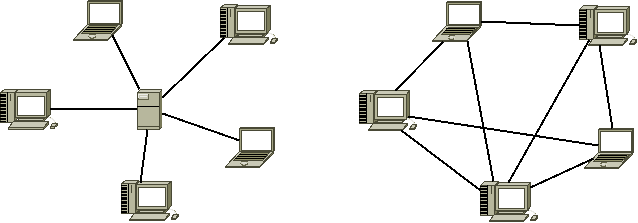
\includegraphics[width=\textwidth]{fig_p2p}
  \caption{Exemple de différence entre une topologie client-serveur et P2P}
  \label{fig:p2p}
\end{figure}

\section{Architecture logicielle}
Afin de suivre le principe \emph{KISS} (Keep It Simple Stupid, \emph{cf.}
Annexe \ref{ann:kiss}) et la philosophie Unix, le projet sera divisé en
plusieurs programmes, chacun d'entre eux s'occupant d'une tâche particulière.
Une autre raison justifiant une telle conception est le fait qu'elle introduit
la possibilité de développer le projet de manière incrémentale, en se
concentrant d'abord sur l'aspect réseau et ensuite sur l'implémentation
propre à un environnement particulier.

\subsection{Client P2P}
Premièrement un logiciel s'occupant uniquement de la gestion du presse-papier
sur le réseau est nécessaire. Celui-ci a comme rôle de se connecter aux
autres pairs et de s'organiser avec ceux-ci quand cela est nécessaire.
Sa seule fonctionnalité est en fait de gérer la partie réseau du système,
toute interaction locale (\emph{i.e.} avec l'utilisateur) se fait par
l'intermédiaire d'autres logiciels qui seront définis par la suite.

Il faut définir de manière plus précise comment l'ensemble des clients P2P
vont s'organiser afin de s'informer pour savoir quel client \emph{détient} le
presse-papier, comment un pair entre dans le réseau et comment détecter
qu'un pair a quitté celui-ci (volontairement ou pas). Des exemples
de fonctionnement de cette architecture et du protocole qui seront mis en
oeuvre sont montrés dans les figures \ref{fig:join} et \ref{fig:copypaste}.

\subsubsection*{Gestion du presse-papier en P2P}
Il y a principalement deux possibilités pour gérer le presse-papier
sur le réseau. Lorsqu'un copier est effectué en local, le client P2P
doit prévenir les autres pairs qu'il détient le presse-papier.
La première option est d'envoyer en même temps la donnée copiée à tous les
pairs. La deuxième est de n'envoyer cette donnée que lorsque qu'un coller
est effectué chez un pair, celui-ci peut alors demander la donnée au pair
détenant le presse-papier.\\\\
La première manière de faire a les avantages et inconvénients suivants:
\begin{itemize}
\item Avantages:
  \begin{itemize}
  \item Possibilité de garder une copie du presse-papier sur chaque pair.
  \item Tolérance aux erreurs dans le cas où le pair détenant le presse-papier
    aurait quitté le réseau.
  \item Absence de communications réseaux en cas de multiples coller.
  \end{itemize}
\item Inconvénients:
  \begin{itemize}
  \item Consommation de bande passante accrue dans le cas où des copiers
    sont effectués fréquemment car il faudra envoyer la même donnée à chacun
    des pairs qui ne feront peut être pas forcément de coller. De plus la
    consommation de bande passante dépend du nombre de pair présent sur le
    réseau.
  \end{itemize}
\end{itemize}
La seconde a les avantages et inconvénients suivants:
\begin{itemize}
\item Avantages:
  \begin{itemize}
  \item Il n'est pas nécessaire de notifier l'ensemble des pairs à chaque
    copier: si un pair effectue plusieurs copies d'affilée, il ne faudrait
    notifier le réseau qu'une seule fois et sans envoyer la moindre donnée.
  \item En général le coller ne sera effectué que par un seul pair,
    il n'a donc qu'à demander lui même au pair détenant le presse-papier
    de la lui envoyer.
  \end{itemize}
\item Inconvénients:
  \begin{itemize}
  \item Impossibilité de récupérer le presse-papier d'un pair ayant quitté
    le réseau.
  \item Si plusieurs collers ont lieu les uns à la suite des autres, il faudra
    demander plusieurs fois la même donnée au pair détenant le presse-papier.\\
  \end{itemize}
\end{itemize}

Il est donc nécessaire de faire un choix entre une de ces options
et c'est la seconde qui est choisie. C'est ainsi que fonctionne non seulement
Remote Clip, mais aussi X Window\cite{nye1992xlib} à la différence
que c'est une architecture client-serveur qui est utilisée. En effet, X Window
est un serveur qui considère chaque fenêtre comme un client. Lorsque
l'utilisateur copie un élément de cette fenêtre, elle notifie le serveur X
qu'elle détient le presse-papier. Ensuite lorsque l'utilisateur
veut coller le contenu du presse-papier, la fenêtre dans laquelle est
effectuée le coller doit demander au serveur X quel client détient le
presse-papier et ensuite s'adresser à celui-ci pour l'obtenir. L'application
devant viser en priorité le monde Unix, c'est ce principe qui est adapté à
une architecture sans serveur. Il faut aussi noter que sous X, il n'est pas
possible de savoir si le presse-papier a changé: si deux copies sont
effectuées au sein de la même application, il n'y a qu'une seule notification
qui est faite auprès des autres fenêtres, il faudrait donc constamment
vérifier que celui-ci a changé ou pas afin de le synchroniser sur le
réseau.

\subsubsection*{Rejoindre le réseau}
Outre un moyen d'authentification, il est nécessaire de définir comment
un pair peut rejoindre le réseau afin de partager son presse-papier.
Pour cela il doit connaître l'adresse IP et l'identifiant d'au moins un pair.
Une fois authentifié, le \emph{parent} contacté lui envoie la liste
des autres pairs faisant partie du réseau en précisant lequel d'entre eux
détient le presse-papier. Une fois cette liste reçue, le \emph{fils}
informe l'ensemble des autres pairs de son arrivée sur le réseau tout en
s'authentifiant auprès de ces pairs. Une fois ceci fait, le pair est considéré
comme faisant partie du réseau et garde chaque connexion ouverte.
Ceci crée une topologie où chaque pair possède une connexion ouverte
avec tous les autres noeuds, ce qui signifie que pour un réseau de $n$
pairs, chaque pair doit maintenir $n-1$ connexions TCP sécurisées. Ceci
pourrait devenir une charge importante à supporter dans un grand réseau, mais
dans notre cas celui-ci est restreint à quelques pairs.

\subsubsection*{Quitter le réseau}
Lorsqu'un pair quitte le réseau, il doit notifier l'ensemble des autres
pairs de son départ. Une fois ceci fait, il peut fermer chaque connexion
ouverte avec chacun des pairs. En revanche il se peut qu'un pair quitte
le réseau sans pouvoir notifier les pairs de son départ, \emph{e.g.}
à cause d'une déconnexion du lien physique. Pour cette raison, lorsqu'un
pair n'est plus joignable, celui-ci est considéré comme sorti du réseau
et la connexion avec celui-ci peut être coupée.

\subsection{Client local}
Le client P2P est le \emph{front-end} avec le réseau, il est chargé
de communiquer avec les pairs du réseau afin de les découvrir et savoir
lequel détient le presse-papier. Le front-end avec l'utilisateur
est en revanche le client local. Celui-ci tourne sur le même ordinateur
que le client P2P, se charge de notifier le client P2P lorsque
l'utilisateur copie quelque chose et le notifie lorsqu'il désire
accéder au presse-papier. Le client P2P notifie le client local
lorsqu'un pair du réseau détient le presse-papier c'est-à-dire lorsque ce
pair effectue un copir.
Un exemple d'interaction entre clients locaux et clients P2P utilisant
le protocole qui sera mis en oeuvre est montré sur la figure \ref{fig:local}.

Cependant, contrairement au client P2P, il peut y avoir plusieurs clients
locaux tournant sur le même ordinateur. Chacun d'entre eux étant destiné
à un environnement précis. Dans ce projet, seront développés deux types
de clients différents:
\begin{itemize}
\item Un client tournant en tâche de fond (comme \emph{daemon}) et
  synchronisant le contenu du presse-papier de X Window.
\item Un client gérant le copier/coller dans un terminal, composé de trois
  logiciels:
  \begin{itemize}
  \item Un daemon gérant le presse-papier, cette fonctionnalité n'étant en
    général pas implémentée dans un shell, seuls les émulateurs de terminaux
    peuvent communiquer avec celui de X Window.
  \item Une commande permettant de copier une donnée à partir de l'entrée
    standard du shell.
  \item Une commande permettant de coller une donnée sur la sortie standard
    du shell.
  \end{itemize}
\end{itemize}
Il est à noter que dans le cas du premier client, le rôle des deux commandes
est en fait joué par les clients X Window \emph{i.e.} les fenêtres ouvertes
et réalisant le copier/coller.

\section{Protocoles}
Deux protocoles sont à définir afin de faire fonctionner l'application
correctement. Le premier est celui utilisé sur le réseau par les clients
P2P afin de communiquer entre eux. Le second est utilisé entre le client
P2P et les clients locaux afin de se notifier mutuellement de changements
dans le presse papier. De même ils doivent tous les deux prendre en compte
l'aspect sécurité, en proposant un moyen d'identification.
Ces deux protocoles seront appelés respectivement protocole P2P et protocole
local.

Les protocoles sont caractérisés par un ensemble de types de messages.
Ceux-ci sont décrits en utilisant la syntaxe suivant:
\begin{verbatim}
MSG <SP> <VAR1> <SP> <VAR2> ... <SP> <VARN> <LF>
\end{verbatim}
MSG définit le type du message. Celui-ci contient $N$ variables
<VAR1>, <VAR2>, $\ldots$, <VARN>. Chacune est séparée par un espace (<SP>)
et le message se termine par un passage à ligne (<LF>). Chaque variable est
ensuite décrite et le type de messages pouvant être reçu comme réponse est
décrit.

\subsection{Protocole P2P}
\subsubsection*{AUTH}
Afin de s'authentifier lors de l'ouverture d'une connexion TCP/TLS,
un identifiant est choisi pour le pair et un mot de passe est défini dans la
configuration du client.
Lorsqu'un pair veut contacter pour la première fois un pair, il doit
s'authentifier auprès de celui-ci. Pour cela il envoie un message
d'authentification:
\begin{verbatim}
AUTH <SP> <NAME> <SP> <PSWD> <LF>
\end{verbatim}
\begin{description}
\item[Variable NAME:] identifiant de l'hôte à joindre.
\item[Variable PSWD:] mot de passe.
\item[Réponse:] si le mot de passe est correct \emph{i.e.} est le même
  utilisé par les deux pairs, le pair contacté peut accepter la connexion
  et répondre par un message de type OK, sinon il répond par un message de type
  KO avec un code d'erreur 1.
\end{description}

\subsubsection*{OK}
Ce type de message permet de confirmer la plupart des opérations:
\begin{verbatim}
OK <LF>
\end{verbatim}

\subsubsection*{KO}
Ce type de message permet de signaler un refus ou une erreur:
\begin{verbatim}
KO <SP> <ERRNO> <LF>
\end{verbatim}
\begin{description}
\item[Variable ERRNO: ] code d'erreur pouvant être:
  \begin{description}
  \item[0] erreur non définie/générique.
  \item[1] échec d'authentification.
  \item[2] pair non valide.
  \end{description}
\end{description}

\subsubsection*{JOIN}
Un message de type JOIN permet de rejoindre le réseau:
\begin{verbatim}
JOIN <SP> <TYPE> <SP> <NAME1> <SP> <NAME2> <LF>
\end{verbatim}
\begin{description}
\item[Variable NAME1:] identifiant du pair.
\item[Variable NAME2:] identifiant du pair contacté.
\item[Variable TYPE:]
  \begin{description}
  \item[0] signifie que le pair n'a pas encore obtenu la liste des pairs
  \item[1] signifie que le pair a déjà la liste des pairs
  \end{description}
\item[Réponse:] si l'identifiant du pair contacté n'est pas le bon, la
  réponse est un message KO avec un code d'erreur 2, si celui-ci est bon la
  réponse est un message de type LIST si le pair a besoin de la liste des
  pairs, sinon un message de type OK.
\end{description}

\subsubsection*{LIST}
Un message de type LIST annonce une liste de messages de type PEER:
\begin{verbatim}
LIST <SP> <N> <LF>
\end{verbatim}
\begin{description}
\item[Variable N:] nombre de messages PEER qui suivent.
\end{description}

\subsubsection*{PEER}
Un message de type PEER décrit ce qui identifie un pair:
\begin{verbatim}
PEER <SP> <NAME> <SP> <IP> <SP> <PORT> <LF>
\end{verbatim}
\begin{description}
\item[Variable NAME:] identifiant du pair permettant d'effectuer un JOIN.
\item[Variable IP:] adresse IP permettant de joindre le pair.
\item[Variable PORT:] port sur lequel le pair écoute.
\end{description}

\subsection*{LEAVE}
Un message de type LEAVE doit être envoyé pour quitter le réseau et ne
nécessite aucune réponse:
\begin{verbatim}
LEAVE <LF>
\end{verbatim}

\subsubsection*{COPY}
Un message de type COPY est envoyé lorsque le pair détient le presse-papier:
\begin{verbatim}
COPY <LF>
\end{verbatim}

\subsubsection*{PASTE}
Un message de type PASTE est envoyé lorsqu'un pair doit obtenir le
presse-papier:
\begin{verbatim}
PASTE <LF>
\end{verbatim}
\begin{description}
\item[Réponse:] Un message de type DATA. Si le pair ne possède pas le
  presse-papier un message de type PEER doit être envoyé avec les informations
  du pair détenant le presse-papier.
\end{description}

\subsubsection*{DATA}
Un message de type DATA permet d'envoyer le contenu du presse-papier:
\begin{verbatim}
DATA <SP> <TYPE> <SP> <LENGTH> <SP> <CONTENT> <LF>
\end{verbatim}
\begin{description}
\item[Variable TYPE:] cette variable permet de préciser le type
  de donnée et ainsi d'étendre facilement le protocole afin de supporter
  d'autres types de données. Dans ce cas il faudra préciser comment ce type
  de données est encodé.
  \begin{description}
  \item[0] type non défini/inconnu.
  \item[1] texte.
  \end{description}
\item[Variable LENGTH:] longueur de la donnée.
\item[Variable CONTENT:] contenu de la donnée dont la longueur
  doit vérifier la variable LENGTH.
\end{description}

\begin{figure}[!h]
  \centering
  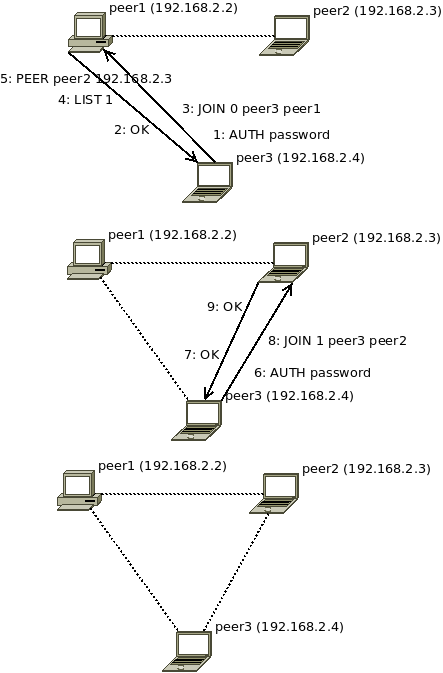
\includegraphics[width=0.9\textwidth]{fig_join}
  \caption{Le pair 3 qui rejoint un réseau. Les lignes en pointillés
    représentent les pairs qui se connaissent mutuellement \emph{i.e.} qui ont
    une connexion TCP/TLS ouverte, et les flèches les communications réseaux
    entre deux pairs. Les messages envoyés sont numérotés afin de suivre
    l'ordre dans lequel ils sont envoyés.}
  \label{fig:join}
\end{figure}

\begin{figure}[!h]
  \centering
  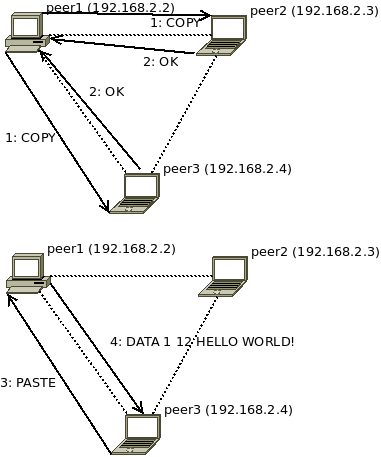
\includegraphics[width=0.9\textwidth]{fig_copypaste}
  \caption{Exemple de copier/coller: le pair 1 copie le texte HELLO WORLD!
    et l'envoie au pair 3 qui fait un coller. Les lignes en pointillés
    représentent les pairs qui se connaissent mutuellement \emph{i.e.} qui ont
    une connexion TCP/TLS ouverte, et les flèches les communications réseaux
    entre deux pairs. Les messages envoyés sont numérotés afin de suivre
    l'ordre dans lequel ils sont envoyés.}
  \label{fig:copypaste}
\end{figure}

\subsection{Protocole local}
Le protocole local utilise un sous-ensemble des messages du protocole P2P,
celui-ci ayant seulement besoin de notifications de copier/coller et de
s'authentifier.
Les messages utilisés seront ceux de type AUTH, OK, KO, COPY, PASTE et DATA.
Les messages de type AUTH, OK et KO sont toujours utilisés pour
l'authentification.

La sémantique des messages de type COPY change légèrement: le client
local envoie un tel message lorsque l'utilisateur copie une donnée dans le
presse-papier et le client P2P envoie un COPY au client local lorsque
c'est un autre pair (ou un autre client local) qui détient le presse-papier.

Les messages de type PASTE sont quant à eux envoyés lorsque le client local
désire faire un coller et qu'il ne détient pas le presse-papier ou bien
lorsqu'un autre pair désire obtenir le contenu du presse-papier détenu par le
client local. Les messages de type DATA ont toujours la même sémantique:
servir de réponse à un message de type PASTE.

\begin{figure}[!h]
  \centering
  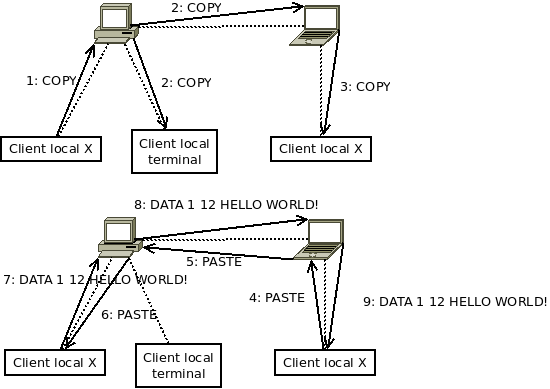
\includegraphics[width=0.9\textwidth]{fig_local}
  \caption{Exemple de copier/coller avec clients locaux. Les lignes en
    pointillés représentent les pairs qui se connaissent mutuellement
    \emph{i.e.} qui ont une connexion TCP/TLS ouverte, et les flèches les
    communications réseaux entre deux pairs. Les messages envoyés sont
    numérotés afin de suivre l'ordre dans lequel ils sont envoyés.}
  \label{fig:local}
\end{figure}

\begin{figure}[!h]
  \centering
  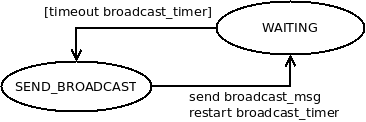
\includegraphics[width=0.9\textwidth]{p2pclient_broadcast}
  \caption{P2P Client Broadcast}
  \label{fig:p2pclient_broadcast}
\end{figure}

\begin{figure}[!h]
  \centering
  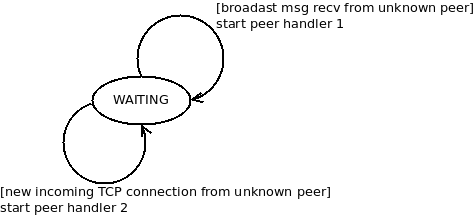
\includegraphics[width=0.9\textwidth]{p2pclient_connections}
  \caption{P2P Client Connections}
  \label{fig:p2pclient_connections}
\end{figure}

\begin{figure}[!h]
  \centering
  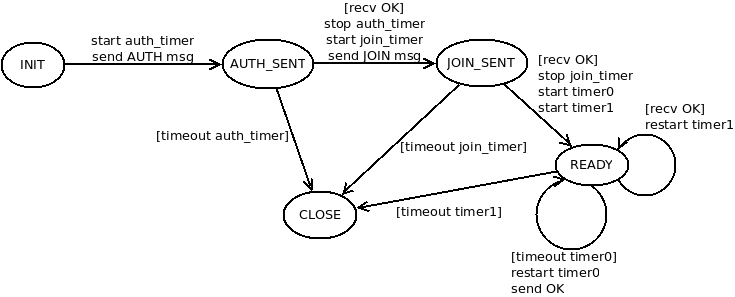
\includegraphics[width=0.9\textwidth]{p2pclient_peerhandler1}
  \caption{P2P Client Peer Handler 1}
  \label{fig:p2pclient_peerhandler1}
\end{figure}

\begin{figure}[!h]
  \centering
  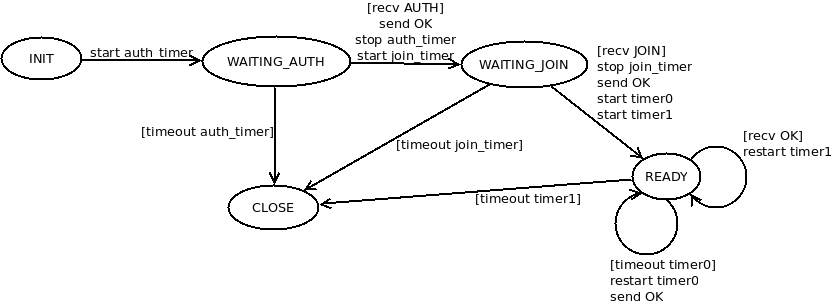
\includegraphics[width=0.9\textwidth]{p2pclient_peerhandler2}
  \caption{P2P Client Peer Handler 2}
  \label{fig:p2pclient_peerhandler2}
\end{figure}

\chapter{Implémentation de la solution proposée}
\renewcommand{\leftmark}{\thechapter.~~Implémentation de la solution proposée}
Ce chapitre justifiera premièrement les choix qui ont été fait avant et
pendant l'implémentationde de l'architecture baptisée \emph{Clipsync}.
Ensuite une présentation de l'utilisation des
logiciels produits sera faite. Après des vérifications de performances seront
effectuées sur ces logiciels et enfin les faiblesses du logiciel seront mises
en avant afin de déterminer les éléments prioritaires à développer lors de
l'évolution future du logiciel.

\section{Choix des outils}
Le langage de programmation C++ a été choisi afin d'implémenter Clipsync,
celui-ci permettant d'avoir un code compilé nativement et ainsi optimisé
pour la machine hôte. Bien que ceci soit une source d'erreurs, il permet
aussi de gérer la mémoire manuellement, ce qui implique un gain de
performances. En revanche les client locaux, à savoir GTKCLip et Shellclip,
ont eux été implémentés en Python. Ce langage de haut niveau en comparaison
au C++ offre la possibilité d'écrire ces deux clients sous forme de scripts
de taille réduite. La perte de performance par rapport au C++ est peu
importante vu que ces scripts utilisent un protocole de communication simple
et servent uniquement d'interface entre l'utilisateur et le client P2P.

La librairie POCO\cite{poco} a été utilisée principalement comme bibliothèque
pour la manipulation de sockets portables. Ceci permet d'avoir une
compatibilité théorique avec Microsoft Windows, bien que celle-ci n'a pas
été testée. De plus POCO offrant un grand nombre de service, la librairie
a aussi été utilisée pour la gestion des threads et des timers, la
configuration du logiciel grâce à un fichier XML, pour la protection de
zones critiques avec mutex, pour la cryptographie et pourla génération de
nombres pseudo-aléatoires.

Afin d'éviter les erreurs en C++, et en particulier les fuites de mémoire,
Valgrind\cite{valgrind} a été utilisé. Celui-ci est à la fois un debugger,
un \emph{memory-checker} et un \emph{profiler}. Celui-ci a permis de debugger
le programme pendant le développement et est utilisé dans la suite de ce
chapitre afin d'analyser les performances du logiciel et pour s'assurer que
le programme n'est pas victime de fuites de mémoires.
Bazaar\cite{bzr} a été utilisé comme gestionnaire de versions décentralisé et
Launchpad\cite{launchpad} a été choisi comme forge sur laquelle déposer le
logiciel produit.

\section{Utilisation des logiciels}
Avant de pouvoir récupérer, compiler et utiliser le logiciel, il est nécessaire
d'avoir les librairies et outils suivants:
\begin{itemize}
\item Bazaar: \url{http://bazaar.canonical.com/}
\item GCC: \url{http://gcc.gnu.org/}
\item GNU Make: \url{http://www.gnu.org/software/make/}
\item POCO version 1.3.6 minimum: \url{http://pocoproject.org/}
\item Python 2.6 ou 2.7: \url{http://www.python.org/}
\item PyGTK et GTK version 2: \url{http://www.pygtk.org/}
\item Doxygen peut être optionnellement installé pour générer la documentation
  du projet: \url{http://www.stack.nl/~dimitri/doxygen/}
\end{itemize}

Tous ces logiciels peuvent êtres installés sous une distribution GNU/Linux
basée sur une Debian récente grâce à la commande:
\begin{verbatim}
sudo apt-get install bzr gcc make libpoco-dev python-gtk2 doxygen
\end{verbatim}

Le code source peut alors être récupéré grâce à la commande:
\begin{verbatim}
bzr branch lp:clipsync
\end{verbatim}
Clipsync peut alors être compilé grâce à GNU Make dans le dossier
\emph{src/clipsync}.
L'exécutable produit peut alors être lancé en passant en paramètre un nom
de fichier XML servant à configurer le logiciel. Un exemple de fichier
est fourni avec le logiciel. Voici la liste des balises et leur description:
\begin{itemize}
\item \emph{net\_frontend}:
  \begin{itemize}
  \item \emph{interface}: interface réseau utilisée pour les communications
    réseau
  \item \emph{use\_ipv6}: booléen servant à indiquer l'utilisation d'IPv6.
    Cette fonctionnalité n'est cependant pas disponible pour le moment et
    l'option a seulement été ajoutée pour l'évolution future du loigiciel.
  \item \emph{port}: port TCP utilisé pour écouter les connexions TCP
    entrantes. C'est sur ce port que le pair sera contacté par les autres
    pairs du réseau.
  \item \emph{bcast\_port}: port UDP utilisé pour l'envoi et la réception de
    messages broadcast.
  \item \emph{bcast\_interval}: interval en millisecondes utilisé pour l'envoi
    de messages broadcast.
  \item \emph{peer\_name}: nom servant à identifier ce pair sur le réseau et
    devant être unique pour ce pair.
  \item \emph{group}: nom du groupe de pairs. Chaque pair du réseau devra
    posséder le même nom de groupe dans sa configuration.
  \item \emph{passphrase} et \emph{salt}: mot de passe et sel\footnote{Le
      salage en cryptographie permet de renforcer la sécurité d'un algorithme
      de chiffrement\cite{wiki:salage}} servant à générer la clé pour le
    chiffrement par AES. Ces deux valeurs doivent être identiques sur chaque
    pair. Il est possible de supprimer ces deux valeurs, de lancer le
    logiciel qui va générer des valeurs aléatoires qui peuvent ensuite
    être copiées sur les autres pairs.
  \item \emph{keepalive\_delay}: délai en millisecondes après lequel la
    connexion est fermée si aucun message OK n'est reçu.
  \item \emph{keepalive\_interval}: interval en millisecondes utilisé pour
    l'envoi de messages OK.
  \item \emph{verbose}, \emph{verbose\_bcast}, \emph{verbose\_peer}:
    booléens permettant d'activer ou de désactiver le mode verbeux
    \footnote{Le mode verbeux permet d'afficher sur la sortie standard
    des informations sur l'activité du logiciel.} de Clipsync.
  \end{itemize}
\item \emph{local\_frontend}:
  \begin{itemize}
  \item \emph{local\_port}: port TCP en local utilisé pour communiquer avec les
    clients locaux.
  \item \emph{verbose}: booléen activant le mode verbeux pour l'interface avec
    les clients locaux.
s  \end{itemize}
\end{itemize}

L'utilisation de Shellclip et GTKClip est possible en exécutant les scripts
Python et en passant en paramètre le port TCP local permettant de contacter
Clipsync.

\section{Vérifications de performances}

\chapter*{Conclusion}
\addcontentsline{toc}{chapter}{Conclusion}
\renewcommand{\leftmark}{CONCLUSION}
Finalement, après avoir examiné le problème, les solutions existantes
pour le résoudre se sont avérées pour la plupart inefficaces. Certaines
ont pourtant de bonnes idées qui ont été reprises afin d'imaginer une
architecture et une ébauche de protocole permettant à des pairs de synchroniser
leur presse-papier sur un réseau. Grâce à cela, il est désormais possible
d'implémenter ce programme afin de fournir une solution efficace.

Pour cela le langage C++ sera utilisé, celui-ci permettant d'avoir un programme
compilé optimisé pour un système précis, il permet de mieux satisfaire
la contrainte de solutions légères qu'avec un langage interprété par une
machine virtuelle. De même le C++ offre l'avantage de donner l'accès
directement à la Xlib et de communiquer facilement avec le serveur
X Window.

La librairie Qt, célèbre pour être utilisée dans l'environnement de bureau
KDE, sera aussi utilisée. Celle-ci permet cependant de faire bien plus que des
programmes fenêtrés. Elle contient entre autre un ensemble de classes
permettant d'établir des connexions TCP/TLS de manière indépendante du
système d'exploitation. Par manque d'expérience avec cette librairie,
il n'est cependant pas possible de dire ce qu'elle pourrait apporter en plus,
celle-ci contenant un grand nombre d'outils différents.

Enfin les prochains mois seront consacrés, tout d'abord à l'étude de
la librairie Qt (et en particulier de sa partie concernant les sockets).
Ensuite une fois ceci fait, il sera possible d'implémenter l'ensemble
des logiciels à fournir de manière incrémentale. Le client P2P sera
d'abord développé afin d'offrir un protocole de base fonctionnel.
Une fois celui-ci implémenté et testé, il sera alors possible
de passer à l'implémentation de trois types de clients locaux.

Un premier permettant une utilisation simple sur l'entrée
et la sortie standard d'un terminal Unix. Le second devra synchroniser le
presse-papier de X Window. Le dernier fournira une interface graphique
basique pour les systèmes ne supportant pas X, il permettra de copier/coller
du texte dans un champ texte et de le synchroniser sur le réseau.
Cependant si une solution est trouvée afin de fournir un client
permettant de synchroniser le presse-papier indépendemment du système
d'exploitation, les deux clients n'en formeront qu'un seul.

%Le style bibliographique utilisé
% \bibliographystyle{latex8}
% \bibliographystyle{alpha}
% \bibliographystyle{alpha}

%Le fichier .bib uitilisé
% \bibliography{biblio}

\printbibliography

\newpage
\appendix
\addcontentsline{toc}{chapter}{Annexes}
\chapter{Codes sources utilisés}\label{ann:src}
\renewcommand{\leftmark}{ANNEXE \thechapter.~~Codes sources utilisés}
\label{annexe1}

Afin de comprendre comment fonctionnent certains logiciels étudiés dans
l'étude de faisabilité, certains codes sources disponibles en ligne
ont été utilisés. Ceux-ci étant disponibles sous licences libres (GPL et MIT),
ils sont non seulement disponibles en ligne mais peuvent aussi être
réutilisés librement.

Bien que ces codes ne seront pas réutilisés pour des raisons évidentes
(utilisation d'un environnement de développement différent), certains
principes ont été compris grâce à ceux-ci. De même les principes de base
utilisé dans le projet s'inspirent largement de ces logiciels, c'est pour
cette raison qu'une annexe leur est consacrée.

\section*{ClipboardMultiSharer}
Le code source Java de l'application sous licence GPL
\footnote{\url{http://sourceforge.net/projects/clipboardmshare/develop}}
a été parcouru afin de comprendre comment fonctionnait
le logiciel, entre autre afin de voir comment il était possible d'accéder
au presse-papier en Java.
La révision consultée était la 16 datant du 10 juillet 2010.

\section*{Clipboard Share}
Bien que disponible sous licence MIT
\footnote{\url{http://clipboardshare.codeplex.com/SourceControl/list/changesets}}, n'ayant pas de connaissances en C\# et en MS .NET, le code de ce logiciel
n'a été ni utilisé dans un but précis, ni lu.

\section*{The Network Clipboard}
Le code source sous licence GPL
\footnote{\url{http://sourceforge.net/projects/netclipboard/develop}}
a été consulté dans le but d'examiner le protocole utilisé. La révision
consultée était la 88.

\section*{Remote Clip}
Le code source sous licence GPL est disponible avec la dernière version
du logiciel
\footnote{\url{http://www.cs.cmu.edu/~rcm/RemoteClip/RemoteClip-3.1.zip}}.
Celui-ci a été consulté dans le but d'étudier le protocole réseau utilisé.

\section*{Gestionnaires de presse-papier}
Le code source de plusieurs gestionnaires de presse-papier ont permis d'aider
à la compréhension du fonctionnement du presse-papier via l'utilisation de
librairies annexes telles que GTK et Qt.
Ces logiciels sont Glipper 2.1\footnote{Version 2.1:
\url{https://launchpad.net/glipper}},
Klipper\footnote{Version présente dans KDE 4.6 (\url{http://www.kde.org})} et
parcellite \footnote{version 1.0.1: \url{http://parcellite.sourceforge.net}}.

\chapter{Principe KISS}\label{ann:kiss}
\renewcommand{\leftmark}{ANNEXE \thechapter.~~Principe KISS}
\label{annexe2}
Le principe \emph{KISS} (Keep It Simple, Stupid!) \cite{wiki:kiss} est un
principe prônant la simplicité, tout particulièrement dans le monde de la
conception.
Il est utilisé dans le développement logiciel dans le but d'exprimer le fait
que la conception doit être simple et éviter toute complexité inutile.

Celui-ci est à la base même de la philosophie Unix, en effet celle-ci prône
l'utilisation de petits utilitaires simples ayant chacun une fonctionnalité
bien précise.
Douglas McIlroy, inventeur du pipe UNIX, a dit\cite{quartercentury-unix}:
\begin{quote}
  This is the Unix philosophy: Write programs that do one thing and do
  it well. Write programs to work together. Write programs to handle
  text streams, because that is a universal interface.
\end{quote}
Le projet a donc été développé en utilisant une approche orientée
composant\cite{wiki:poc}, en fournissant de petits
logiciels communiquant au travers de sockets de manière textuelle.

Plusieurs auteurs
\cite{Brooks1995, Raymond2001} prônent cette philosophie sans pour autant
y faire référence explicitement. \emph{e.g.} Brooks explique par exemple
que le design est d'une importance capitale car il permet de comprendre
plus facilement le code source, Raymond dit qu'il faut concevoir les logiciels
de manière à ce qu'ils suivent la philosophie d'Unix. Il dit aussi que
la perfection en conception n'est pas atteinte lorsque l'on n'a plus rien à
ajouter mais plutôt lorsque l'on n'a plus rien à retirer.

Filip Hanik, un ingénieur logiciel membre de l'\emph{Apache Foundation} parle
aussi du principe KISS et donne des conseils pour appliquer ces principes en
Java (mais ceux-ci sont applicables dans tous les langages de programmation)
\cite{fhanikKISS}.


\end{document}
